


\chapter{Introduction}\paragraph{}Understanding the world around us is the goal of every scientist, from the chemist that experiments with the formation of atoms to the geologist exploring the process of rock formations. Nuclear physicists focus on studying the fundamental constituents of matter, the building blocks of nature. Physicist use scattering experiments at accelerator facilities, like CERN in Switzerland, DESY in Germany, BATES in Massachusetts, JLAB in Virgina, and many others, to study the protons and neutrons and their constituents that make up a nucleus. These experiments allow physicists to observe the internal structure of the nucleus and to investigate the interactions between the quarks and gluons. Many of the experiments are design to confirm a existing results while also expanding on unique ideas.
\paragraph{}In the last century, there have been numerous breakthroughs in the fields of nuclear and particle physics. Rutherford discovered the proton by bombarding light nuclei with alpha particles to produce 
	\begin{equation}
	^{14}N + ^4He \rightarrow ^{17}O + p.
	\end{equation}
This reaction allowed Rutherford to conclude that the Hydrogen nucleus was a constituent of an atomic nuclei \cite{PnN}. In the late 1950s, experimental results published by W. McAllister and R. Hofstadter exposed some of the eternal structure of the proton \cite{Flay,Hof}. The European Muon Collaboration(EMC) produced results in the early 1980s showing a differences between the internal structure of the deuterium nucleus and Iron \cite{seeley,CC}. The data received from scattering experiments using alpha particles contain information about the target, the beam, and the interaction between the two. Deciphering and analyzing this data can be convoluted because the cross-section contains information about the internal structure of the target and the beam along with the interaction and forces between the two \cite{PnN}.  

\section{Electron scattering}
\paragraph{} In order to remove some of the complexity in scattering experiments, one may employ highly relativistic electrons. Electrons being point-like particles without any internal structure allow the elimination of some of the analysis difficulties with using alpha particles in scattering experiments due to their complex internal structure. Electrons and the target nucleus, nucleon, or quarks interact via the exchange of a virtual photon. Using quantum electrodynamics (QED), these interactions can accurately be described by the well known electromagnetic interaction. Higher order terms of this process contribute very little due to the coupling constant $\alpha \approx 1/137 $, being much smaller than one. 
\paragraph{} Figure \ref{feynman} represents an electron scattering from a proton. The incoming or incident electron's four-momentum is described as k = (E,$ \vec{k}$) and the scattering electron's four-momentum is represented by $k^\prime{}$ = ($E^\prime{}$,$\vec{k}^\prime{}$). The exchange of the virtual photon in this electromagnetic interaction is defined by the four-momentum transfer q: 
\begin{equation}
\label{Q}
Q^2 \equiv -q^2 = 4EE^\prime{} sin^2(\theta/2).
\end{equation} 
In equation \ref{Q}, E and E$^\prime$ are the electron energy before and after the scattering interaction. Theta is the angle that describes the deflection of E$^\prime$ from the electron's original path. 

\begin{figure}[h]
\centering
\caption{Simple Feynman diagram of an electron scattering from a proton \cite{Flay}.}
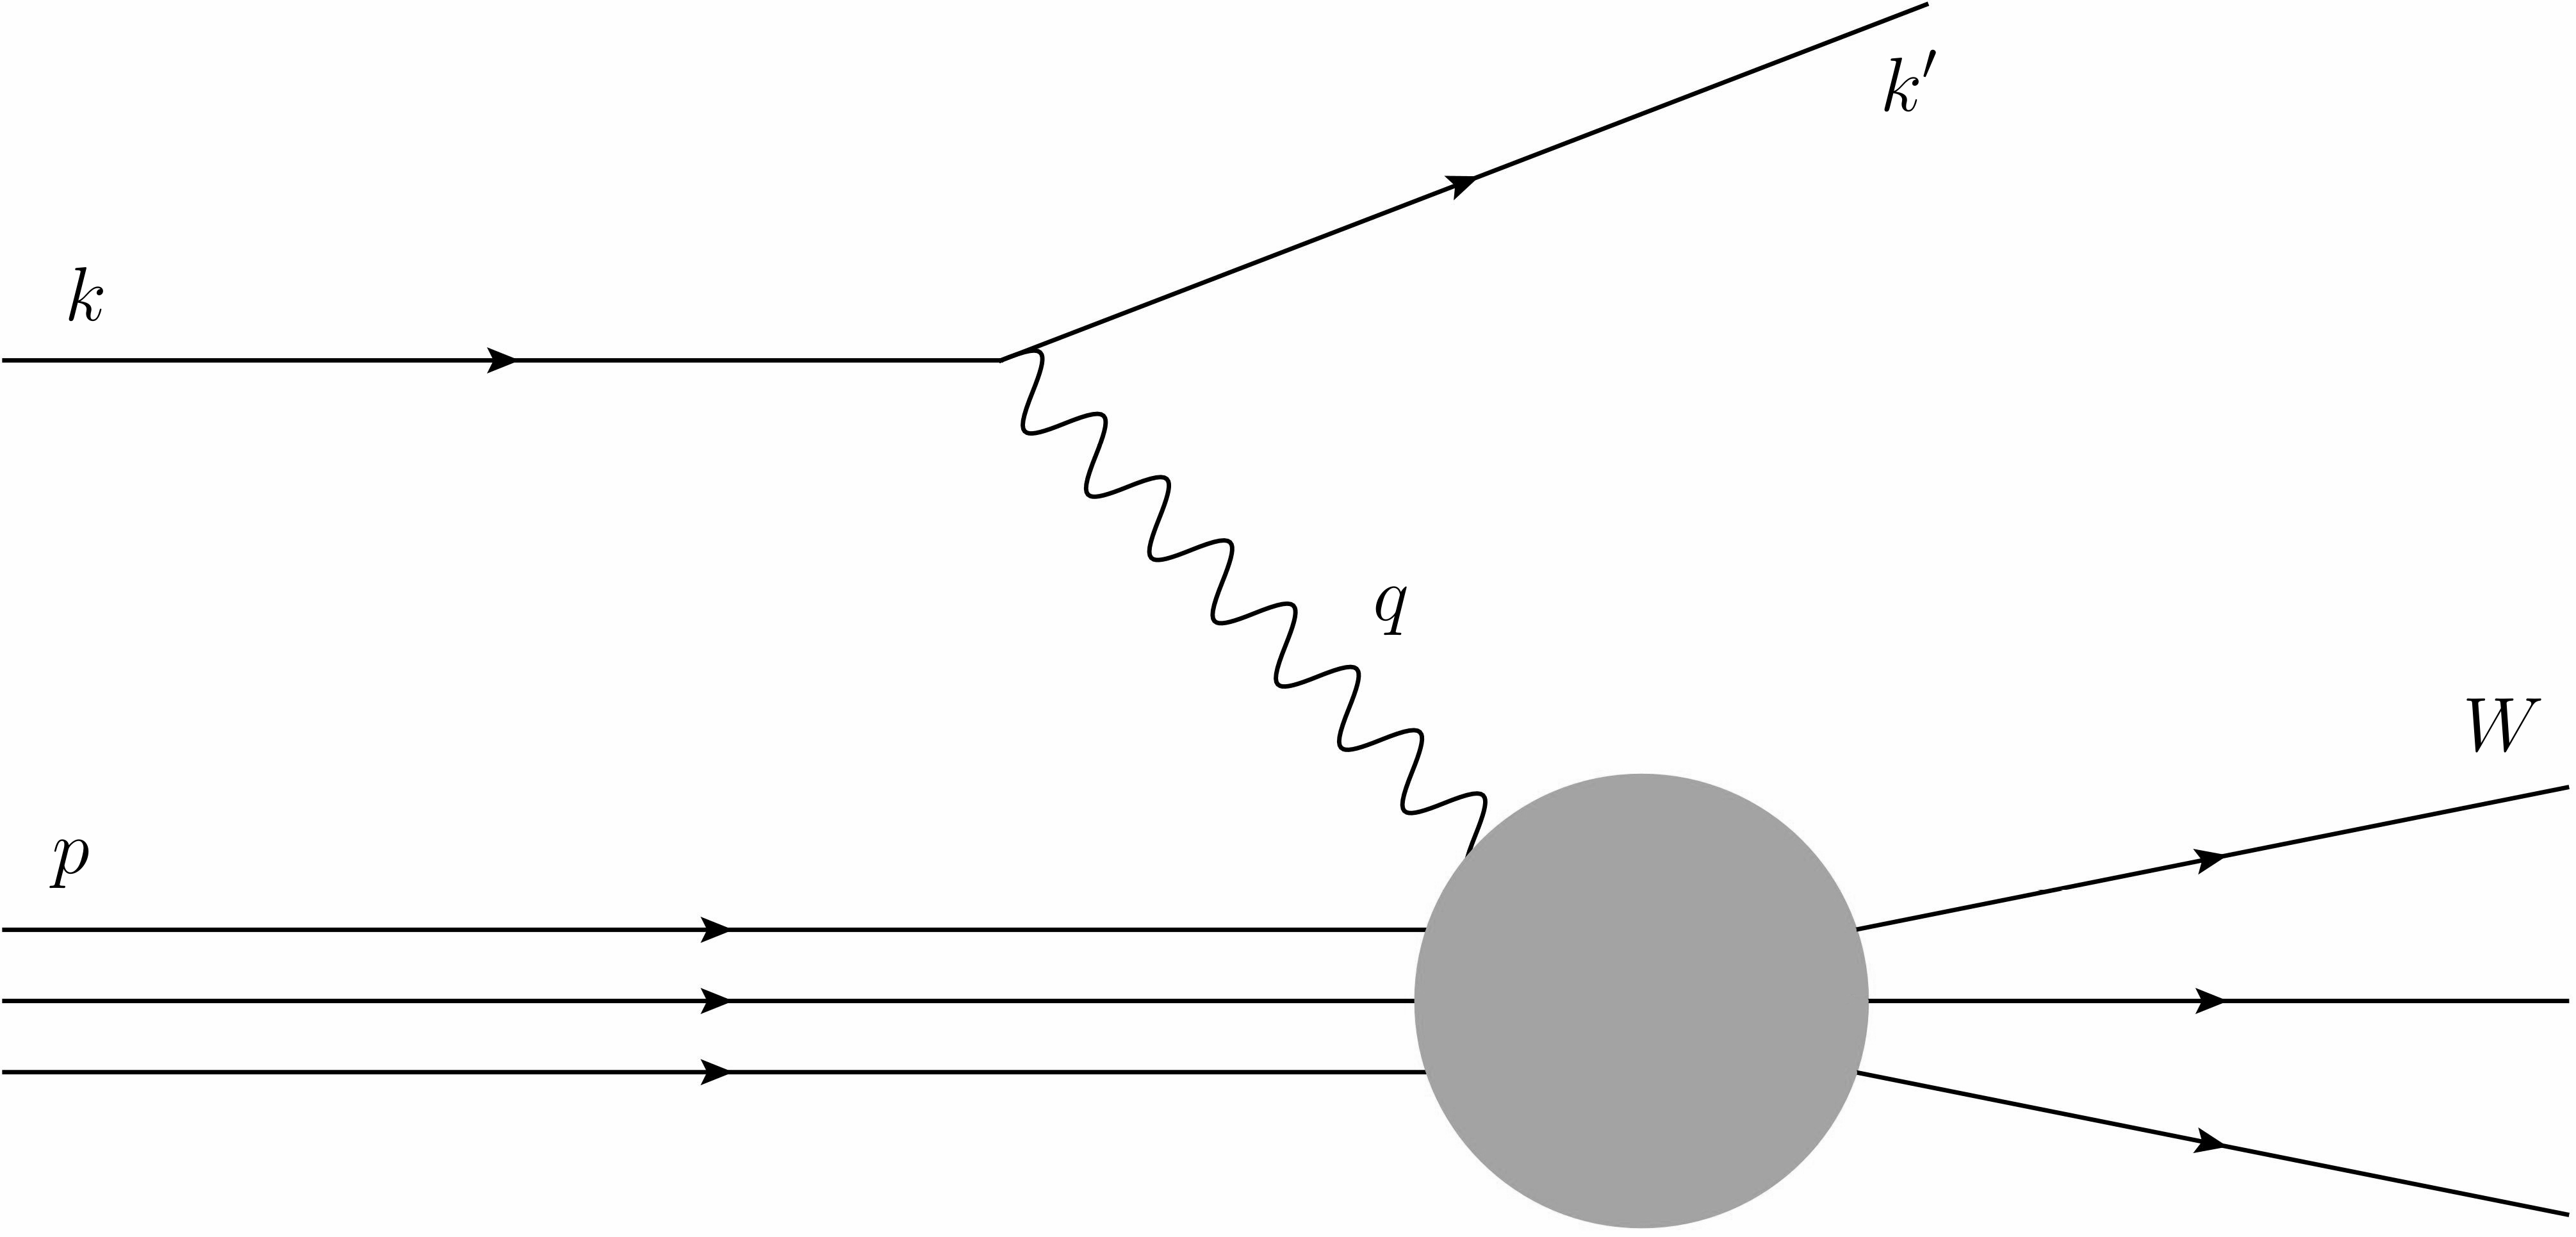
\includegraphics[width=10cm]{feyman_e_p.png}
\label{feynman}
\end{figure}
Along with $Q^2$, the variables $\nu$, W, and$x_B$  are used to narrate the evolution of the electron scattering process. $\nu$, defined as $p\cdot q/M$. In the rest frame of the target,  $\nu$ can be described by:

\begin{equation}
\label{v}
\nu = E - E^\prime{}.
\end{equation}
Simply, $\nu$ is the magnitude of energy loss by the electron during the scattering interaction. The invariant mass of the system, W,  defines the hadronic state produced by the scattering event. 
\begin{equation}
\label{W}
W^2 \equiv (q + p)^2 = M^2 + 2M\nu -Q^2.
\end{equation}
A scattering event with the invariant mass equal to the square of the mass of the nucleon, ($M^2$), falls in the regime of elastic scattering. W above $M^2$ will transform the scattering interaction from an elastic scattering to inelastic scattering due to the excited state of the scattered byproduct. $x_B$, the Bjorken scaling variable is a dimensionless quantity that measures the inelastically of a scattering process. $x_B$ is defined as: $x := \frac{Q^2}{2M\nu}$.
\paragraph{} The intrinsic likelihood of an event with a certain $Q^2$, $\nu$, and $W$ is defined by the scattering cross section. An electron scattering off of a target with a charge of $Z*e$ can be described by the Rutherford cross-section. Povh et. al. details the Rutherford cross section as:
\begin{equation}
\bigg(\frac{d\sigma}{d\Omega}\bigg)_{Rutherford} = \frac{ \big(zZe^2\big)^2} {\big( 4\pi \epsilon_0\big)^2 * \big(e E_{kin}\big)^2 sin^4\big( \theta / 2 \big) }. 
\end{equation}
  In the early 1920s, German physicists Stern and Gerlach performed an experiment that confirmed the presence of electron angular momentum. Later a discovery of electron spin was made by Uhlenbeck an Gloudsmit.  The Rutherford cross-section neglects the spin of a electron and it's target. The Mott cross-section is the evolved version of the Rutherford cross-section. It has been modified to include the intrinsic spin of the target and electron. The Mott cross-section is: \cite{HighE,PnN}
\begin{equation}
\bigg(\frac{d\sigma}{d\Omega}\bigg)_{Mott} = \frac{4Z^2\alpha^2 \big(\hbar c \big)^2 E{^{\prime} }^2}{ |\boldsymbol{q}c|^4} cos^2 (\theta/2).
\end{equation}

\paragraph{}There is an agreement between the measured cross section and the theoretical Mott cross-section when in the limit of $|\boldsymbol{q}| \rightarrow  0$ for scattering events of electrons off of a target nuclei. As $|\boldsymbol{q}|$ climbs furtherer from zero, the experimentally measured cross sections systematically decreases \cite{PnN}. Increasing the $|\boldsymbol{q}|$ of an interaction reduces the size of the wavelength of the virtual photon that mediates the electromagnetic interaction between the electron and target nuclei and increases the resolution of the probe. The wavelength of this virtual photon is inversely proportional to $|\boldsymbol{q}|$, and can be described by the following: $\lambda = \ \frac{\hbar}{|\boldsymbol{q}|}$ \cite{PnN}. Increasing the amount of momentum transfered in an electromagnetic reaction allows one to study deeper into the nucleus. 
\paragraph{} Studying the internal structure of a nucleus with the electromagnetic interaction requires increasing the momentum transfered. Pushing $|\boldsymbol{q}|$ to be comparable with the mass of a nucleon adds more complexity to the details of the scattering interaction. At the appropriate levels of $|\boldsymbol{q}|$ to study the nucleons in the nucleus, the Mott cross-section equation requires modifications to include additional factors that incorporate information about the target. The Rosenbluth formula is based on the Mott cross section and embraces target recoil, magnetic moment, and charge and current distributions. Povh writes the Rosenbluth formula as:
\begin{equation}
\label{rosen}
\bigg(\frac{d\sigma}{d\Omega}\bigg)=\bigg(\frac{d\sigma}{d\Omega}\bigg)_{Mott} *\bigg\lbrack \frac{G^2_E(Q^2) +\tau G^2_M(Q^2)}{1+\tau} + 2\tau G^2_M(Q^2)tan^2\frac{\theta}{2} \bigg\rbrack.
\end{equation}
Equation \ref{rosen} contains $G^2_E(Q^2)$ and $G^2_M(Q^2)$, the electric and magnetic form factors. $\tau$ is used in the Rosenbluth formalism to account for the magnetic moment of a nucleon and is defined as: $\tau = \frac{Q^2}{4M^2c^2}$ \cite{PnN}. In the general case of electron scattering off of a free proton or neutron elastically, the scattered energy of the electron will be a function of the incident electron's energy and the scatted angle of the electron, shown in the following equation.
\begin{equation}
E^\prime =\frac{E}{1+\frac{E}{Mc^2}(1-cos\theta)}
\end{equation}
\subsection{Deep inelastic scattering}
\paragraph{}The first generation of electron scattering experiments achieving a significantly large  $|\boldsymbol{q}|$ used a linear accelerator with a 25 GeV maximum beam energy, and following generations increased the total interaction energy to substantially higher thresholds. At these high incident beam energies, individual resonances cannot be separated in the invariant mass spectrum above 2.5 GeV. Observations made into this convoluted invariant mass spectrum has shown that many strongly interacting particles are produced, known as hadrons. Scattering interactions that generate these hadrons are considered to be inelastic. Inelastic scattering events contain the possibility of conceiving additional resultants and increase the complexity of a scattering interaction. Inelastic scattering events occur when the wavelength of the virtual photon is comparable to the radius of the struck nucleon or when $Q^2R^2 \lesssim 1$\cite{PnN}. Increasing the amount of transferred momentum so that $Q^2R^2 \gtrsim 1$, increase the resolution of the probe to a level that allows for the interacting with the charge constituents within the nucleon. When the scattering event probes the fundamental elements of a nucleon, the scattering process is titled deep inelastic scattering(DIS). Due to the increase in complexity, an additional degree of freedom has to be introduced into the scattering cross section equation. Modifying the Rosenbluth formula to include the inelastic scattering structure functions $F_1(Q^2,\nu)$ and $F_2(Q^2,\nu)$ evolves the Rosenbluth formula to contain the needed complexity of an inelastic event. These modifications are shown in equation \ref{ISCS}.
\begin{equation}
\label{ISCS}
\frac{d^2\sigma}{d\Omega dE^\prime}=\bigg(\frac{d\sigma}{d\Omega}\bigg)_{Mott} \bigg\lbrack \frac{F_2(Q^2,\nu)}{\nu} + \frac{2F_1(Q^2,\nu)}{M}tan^2\frac{\theta}{2} \bigg \rbrack
\end{equation}  

The $F_1$ and $F_2$ structure functions provide the details for describing the internal composition of the nucleon \cite{PnN}. 
\begin{equation}
\label{F2q}
F_2(x) = x1 \cdot \Sigma_f z^2_f ( q_f(x) + \bar{q}_f(x))
\end{equation}

	

	\cite{DISearly}
	\cite{DISproton}

	
\section{EMC Effect}
\paragraph{}The European Muon Collaboration (EMC) performed a deep inelastic measurement with 120-280 GeV muons on iron and deuteron targets \cite{challenge}. The EMC extracted A/D structure function ratios versus the Bjorken scaling variable, $x$.  The relationship originally expected by the EMC contained the sum of the structure functions of each nucleon in a nucleus. Each nucleus has a certain number of neutrons (N) and a amount of protons (Z). The expected structure function for a nucleus could be written as:
\begin{equation}
F_A = N F_2^N + ZF_2^P.
\end{equation}
 The EMC compared the extracted structure functions from iron and deuterium. Their results are shown in Figure \ref{EMCOld}. The $\frac{A}{D}$ structure function ratio showed an unexpected downward slope. This phenomenon was titled the EMC effect. This finding demonstrated to the EMC that their understanding of the nucleus was incorrect. A nucleon's structure function and thereby, the constituent quark distributions may be altered by the nucleus. 
\begin{figure}[h]
\centering
 \caption{ Graph of the ratio of A/D structure functions vs $x$ for Carbon \cite{CC}.}
 \label{EMCOld}
 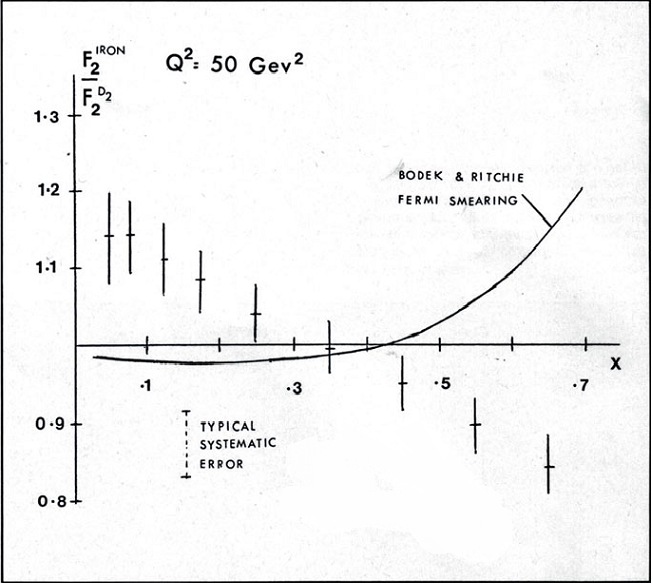
\includegraphics[width=10cm]{EMC.png} 
 \end{figure} 

\paragraph{}Ever since the European Muon Collaboration discovered the depletion of quarks at high $x$ for A $>$2 nuclei, physicists have tried to discover its cause. Scientists at SLAC extracted structure function ratios for many nuclei including; $^4$He, $^9$Be, $^{12}$C, $^{27}$Al, $^{40}$Ca, $^{56}$Fe, $^{108}$Ag, and $^{197}$Au. There were slightly different results for each nucleus. The magnitude of the EMC effect, taken to be the A/D ratio at $x=0.6$, was found to be different for the various nuclei, and roughly scaled with the size or density of the nuclei. The NMC (New Muon collaboration), another group at CERN, gathered precise data in order to construct the inclusive cross section of deuterium and protons. BCDMS collaboration extracted data for N and Fe structure function ratios. Figure \ref{EMC3} shows some of the data from SLAC and BCDMS on the EMC effect for Iron and Cu. Figure \ref{EMC 1} shows this result from a recent JLab EMC measurement, most precise to date. Many models over the years have been able to reproduce the shape of the A/D ratios. These models can contain traditional nuclear physics effects like momentum distribution or pion-charge contributions. Some models also describe the EMC effect through quark momentum distribution or modification of the internal structure \cite{Norton, piler, arri, DF, gomez}. However, no single model has provided a complete picture of the possible underlying physics. Precise data from Jlab's E03-103 experiment has revitalized this research. This experiment focused on precision measurements in light nuclei and added $^{3}$He as a target nucleus. Instead of taking the A/D ratio at a certain $x$-value to be the magnitude of the EMC effect, this analysis looked at the slope instead. This eliminated sensitivity to normalization uncertainties.

\begin{figure}[h]
\centering
\caption{EMC effect from EMC, SLAC, and BCDMS \cite{Norton}}
\label{EMC3}
\centering
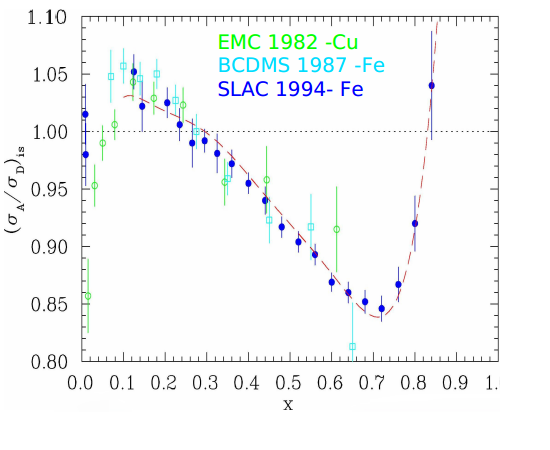
\includegraphics[width=10cm]{EMC3.png}
\end{figure}

\begin{figure}[h]
\centering
 \caption{ Graph of the ratio of A/D structure functions vs $x$ for Carbon \cite{CC}.}
 \label{EMC 1}
 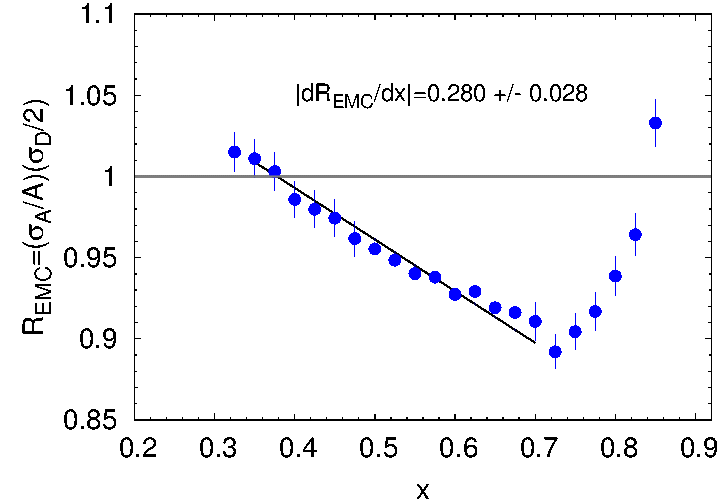
\includegraphics[width=10cm]{EMC1.png} 
 \end{figure} 
 

\paragraph{} In Figure , $^9$Be was found not to follow the previously observed scaling with nuclear density. This result from Jefferson Lab determined that the previous idea of a dependence on A or nuclear density in the EMC effect to be incorrect \cite{seeley}. This result spawned a drive to determine another explanation for the EMC effect and understand what clue the $^9$Be outlier was providing. The structure of this nucleus is made up of two high-density alpha particles and a single neutron \cite{ajppt}. The regions of higher density that are contained in a comparatively large volume may be able to explain why $^9$Be does not follow the expected trend. This suggests that the EMC effect could be a function of local nuclear density \cite{seeley}. 




\section{MARATHON}
Experiment E12-010-102, MARATHON (MeAsurement of the $F2^n$/$F_2^p$,$d$/$u$ RAtios and A=3 EMC Effect in Deep Inelastic Electron Scattering Off the Tritium and Helium MirrOr Nuclei), will use deep inelastic scattering off of the mirror nuclei $^3$H and $^3$He to measure the EMC effect for both $^3$H and $^3$He, to determine the ratio of the neutron to proton inelastic structure functions, and to find the ratio of the down to up quark distributions in the nucleon.

